\documentclass[]{article}

\usepackage{hyperref}
\usepackage{graphicx}
\usepackage{mathtools}
\usepackage{amssymb}
\usepackage{algorithm2e}
\usepackage[T1]{fontenc}
%\usepackage{enumitem}
\usepackage{paralist}
\usepackage{csquotes}
\usepackage[affil-it]{authblk}
\usepackage{listings}
\usepackage{fixltx2e}
\usepackage[numbers]{natbib}
\usepackage{mathpartir}
\usepackage{mmm}

% Treat paragraph as subsubsubsection
\usepackage{titlesec}
\setcounter{secnumdepth}{4}

\usepackage{tikz}
\usetikzlibrary{shapes,arrows,decorations.pathreplacing,calc}

\DeclareMathOperator{\md5}{MD5}

\lstset{
  frame=none,
  xleftmargin=2pt,
  stepnumber=1,
  numbers=none,
  numbersep=5pt,
  numberstyle=\ttfamily\tiny\color[gray]{0.3},
  columns=flexible,
  belowcaptionskip=\bigskipamount,
  captionpos=b,
  escapeinside={*'}{'*},
  language=haskell,
  tabsize=2,
  emphstyle={\bf},
  commentstyle=\it,
  stringstyle=\mdseries\ttfamily,
  showspaces=false,
  keepspaces=true,
  keywordstyle=\bfseries\ttfamily,
  basicstyle=\small\ttfamily,
  showstringspaces=false,
  morecomment=[l]\%,
}

\newcommand{\fc}{System F\textsubscript{C}}

\newcommand{\qcheck}{\textsc{QuickCheck}}
\newcommand{\qspec}{\textsc{QuickSpec}}
\newcommand{\hspec}{\textsc{HipSpec}}

\providecommand{\hs}[1]{\lstinline[language=Haskell]|#1|}

\providecommand{\coq}[1]{\lstinline[language=ML]|#1|}

\lstnewenvironment{haskell}{%
  \lstset{language=Haskell, xleftmargin=.2\textwidth, xrightmargin=.2\textwidth}}{}

\lstnewenvironment{coqblock}{%
  \lstset{language=ML, xleftmargin=.2\textwidth, xrightmargin=.2\textwidth}}{}

\begin{document}

\pagestyle{headings}  % switches on printing of running heads

\title{Improving Haskell Theory Exploration}

\author{Chris Warburton}

\affil{University of Dundee,\\
\texttt{http://tocai.computing.dundee.ac.uk}}

\maketitle              % typeset the title of the contribution

\begin{abstract}
Theory Exploration is a promising approach to improving the quality and understanding of software, above that available through testing, in languages which are amenable to formal analysis such as those based on pure functional programming. Current techniques are limited by their computational cost, which we mitigate through a divide and conquer approach: reducing the problem size whilst using a machine learning approach to preserve relevant details.
\end{abstract}

\section{Introduction}

\iffalse
TODO
Intro + motivation

About 2 pages

Haskell is a mainstream FP language (motivation)

QuickCheck (example)

How to come up with the properties

Mention theory exploration
\fi

As computers and software become more capable, and as our reliance on them increases, the importance of \emph{understanding}, \emph{predicting} and \emph{verifying} these systems grows; which is undermined by their ever-increasing complexity. The \emph{functional programming} paradigm has been proposed for addressing these issues \cite{hughes1989functional}, in part by constructing programs which are more amenable to mathematical analysis. For example, by separating \emph{computation} from \emph{effects}, we can analyse each in isolation; in particular, pure computations can be evaluated without fear of damaging side-effects, and results are repeatable (since there can be no dependence on external state).

Whilst use of pure functional programming languages, like Haskell and Idris, is relatively rare, their features are well suited to common software engineering practices like \emph{unit testing}; where tasks are broken down into small, easily-specified ``units'', and tested in isolation for a variety of use-cases. Functional ideas are thus spreading to mainstream software engineering in a more dilute form; seen, for example, in the recent inclusion of first-class functions in Java \cite{gosling2015java} and C++ \cite{willcock2006lambda}.

Functional programming is also well suited to more radical practices, such as \emph{property checking} and \emph{theorem proving}, which are promising methods for increasing confidence in software, yet are currently prohibitively expensive. Here we investigate how the recent \emph{theory exploration} approach can lower the effort required to pursue these goals, and in particular how machine learning techniques can mitigate the costs of the combinatorial algorithms involved.

\iffalse
TODO
Our contributions are:

\begin{itemize}
  \item A framework for applying theory exploration tools such as \qspec{} to Haskell's existing package system.
  \item A
\end{itemize}
\fi

\section{Background}
\label{sec:background}

\subsection{Haskell}
\label{sec:haskell}

\begin{figure}
  \begin{equation*}
    \begin{split}
      expr\    \rightarrow\ & \texttt{Var}\ id                                       \\
                         |\ & \texttt{Lit}\ literal                                  \\
                         |\ & \texttt{App}\ expr\ expr                               \\
                         |\ & \texttt{Lam}\ \mathcal{L}\ expr                        \\
                         |\ & \texttt{Let}\ bind\ expr                               \\
                         |\ & \texttt{Case}\ expr\ \mathcal{L}\ \left[ alt \right]   \\
                         |\ & \texttt{Type}                                          \\
      id\      \rightarrow\ & \texttt{Local}\ \mathcal{L}                            \\
                         |\ & \texttt{Global}\ \mathcal{G}                           \\
      literal\ \rightarrow\ & \texttt{LitNum}\ \mathcal{N}                           \\
                         |\ & \texttt{LitStr}\ \mathcal{S}                           \\
      alt\     \rightarrow\ & ( altcon,\ [\mathcal{L}],\ expr )                      \\
      altcon\  \rightarrow\ & \texttt{DataAlt}\ \mathcal{G}                          \\
                         |\ & \texttt{LitAlt}\ literal                               \\
                         |\ & \texttt{Default}                                       \\
      bind\    \rightarrow\ & \texttt{NonRec}\ \mathcal{L}\ expr                     \\
                         |\ & \texttt{Rec}\ [ ( \mathcal{L},\ expr ) ]
    \end{split}
  \end{equation*}
  Where:
  \begin{tabular}[t]{l @{ $=$ } l}
    $\mathcal{S}$ & string literals    \\
    $\mathcal{N}$ & numeric literals   \\
    $\mathcal{L}$ & local identifiers  \\
    $\mathcal{G}$ & global identifiers
  \end{tabular}

  \caption{Simplified syntax of GHC Core in BNF style. $[]$ and $(,)$ denote repetition and grouping, respectively.}
  \label{fig:coresyntax}
\end{figure}

We decided to focus on theory exploration in the Haskell programming language as it has mature, state-of-the-art implementations (\qspec{} \citep{QuickSpec} and \hspec{} \citep{claessen2013automating}). This is evident from the fact that the state-of-the-art equivalent for Isabelle/HOL, the \textsc{Hipster} \citep{Hipster} system, is actually implemented by translating to Haskell and invoking \hspec{}.

Haskell is well-suited to programming language research; indeed, this was a goal of the language's creators \citep{marlow2010haskell}. Like most members of the \emph{functional programming} paradigm, Haskell is essentially a variant of $\lambda$-calculus, with extra features such as a strong type system and ``syntactic sugar'' to improve readability. For simplicity, we will focus on an intermediate representation of the \textsc{GHC} compiler, known as \emph{GHC Core}, rather than the relatively large and complex syntax of Haskell proper. Core is based on \fc{}, but for our machine learning purposes we are mostly interested in its syntax; for a more thorough treatment of \fc{} and its use in GHC, see \citep[Appendix C]{sulzmann2007system}.

The sub-set of Core we consider is shown in figure \ref{fig:coresyntax}; compared to the full language \footnote{As of GHC version 7.10.2, the latest at the time of writing.} our major changes are to ignore type hints (explicit casts are removed, whilst particular types/kinds/coercions are all represented by \texttt{Type}) and to use a custom representation of names. We also omit several other forms of literal (machine words of various sizes, individual characters, etc.) for brevity, as their treatment is similar to those of strings and numerals.

\subsection{QuickCheck}
\label{sec:quickcheck}

Although unit testing is the de facto industry standard for quality assurance in non-critical systems, the level of confidence it provides is rather low, and totally inadequate for many (e.g. life-) critical systems. To see why, consider the following Haskell function, along with some unit tests:

\begin{lstlisting}[language=Haskell, xleftmargin=.2\textwidth, xrightmargin=.2\textwidth]
factorial 0 = 1
factorial n = n * factorial (n-1)

fact_base      = factorial 0 == factorial 1
fact_increases = factorial 3 <= factorial 4
fact_div       = factorial 4 == factorial 5 `div` 5
\end{lstlisting}

The intent of the function is to map an input $n$ to an output $n!$. The tests check a few properties of the implementation, including the base case, that the function is monotonically increasing, and a relationship between adjacent outputs. However, these tests will \emph{not} expose a serious problem with the implementation: it diverges on half of its possible inputs!

All of Haskell's built-in numeric types allow negative numbers, which this implementation doesn't take into account. Whilst this is a rather trivial example, it highlights a common problem: unit tests are insufficient to expose incorrect assumptions. In this case, our assumption that numbers are positive has caused a bug in the implementation \emph{and} limited the tests we've written.

If we do manage to spot this error, we might capture it in a \emph{regression test} and update the definition of \hs{factorial} to handle negative numbers, e.g. by taking their absolute value:

\begin{lstlisting}[language=Haskell, xleftmargin=.2\textwidth, xrightmargin=.2\textwidth]
factorial 0 = 1
factorial n = let nPos = abs n
               in nPos * factorial (nPos - 1)

fact_neg = factorial 1 == factorial (-1)
\end{lstlisting}

However, this is \emph{still} not enough, since this function will also accept fractional values\footnote{Since we only use generic numeric operations, the function will be polymorphic with a type of the form \hs{forall t. Num t => t -> t}, where \hs{Num t} constrains the type variable \hs{t} to be numeric. In fact, Haskell will infer extra constraints such as \hs{Eq t} since we have used \hs{==} in the unit tests.}, which will also cause it to diverge. Clearly, by choosing what to test we are biasing the test suite towards those cases we've already taken into account, whilst neglecting the problems we did not expect.

Haskell offers a partial solution to this problem in the form of \emph{property checking}. Tools such as \qcheck{} separate tests into three components: a \emph{property} to check, which unlike a unit test may contain \emph{free variables}; a source of values to instantiate these free variables; and a stopping criterion. Here is how we might restate our unit tests as properties:

\begin{lstlisting}[language=Haskell, xleftmargin=.2\textwidth, xrightmargin=.2\textwidth]
fact_base        = factorial 0 == factorial 1
fact_increases n = factorial n <= factorial (n+1)
fact_div       n = factorial n == factorial (n+1) `div` (n+1)
fact_neg       n = factorial n == factorial (-n)
\end{lstlisting}

The free variables (all called \hs{n} in this case) are abstracted as function parameters; these parameters are implicitly \emph{universally quantified}, i.e. we've gone from a unit test asserting $factorial(3) \leq factorial(4)$ to a property asserting $\forall n, factorial(n) \leq factorial(n+1)$. Notice that unit tests like \hs{fact_base} are valid properties; they just assert rather weak statements.

To check these properties, \qcheck{} treats closed terms (like \hs{fact_base}) just like unit tests: pass if they evaluate to \hs{True}, fail otherwise. For open terms, a random selection of values are generated and passed in via the function parameter; the results are then treated in the same way as closed terms. The default stopping criterion for \qcheck{} (for each test) is when a single generated test fails, or when 100 generated tests pass.

The ability to state \emph{universal} properties in this way avoids some of the bias we encountered with unit tests. In the \hs{factorial} example, this manifests in two ways:

\begin{itemize}
  \item \qcheck{} cannot test polymorphic functions; they must be \emph{monomorphised} first (instantiated to a particular concrete type). This is a technical limitation, since \qcheck{} must know which type of values to generate, but in our example it would bring the issue with fractional values to our attention.

  \item The generators used by \qcheck{} depend only on the \emph{type} of value they are generating: since \hs{Int} includes positive and negative values, the \hs{Int} generator will output both. This will expose the problem with negative numbers, which we weren't expecting.
\end{itemize}

Property checking is certainly an improvement over unit testing, but the problem of tests being biased towards expected cases remains, since we are manually specifying the properties to be checked.

We can reduce this bias further through the use of \emph{theory exploration} tools, such as \qspec{} and \hspec{}. These programs \emph{discover} properties of a ``theory'' (e.g. a library), through a combination of brute-force enumeration, random testing and (in the case of \hspec{}) automated theorem proving.

\subsection{Theory Exploration}
\label{sec:theoryexploration}

\newcommand{\blank}{\cdot}

In this work we consider the problem of \emph{(automated) theory exploration}, which includes the ability to \emph{generate} conjectures about code, to \emph{prove} those conjectures, and hence output \emph{novel} theorems without guidance from the user. The method of conjecture generation is a key characteristic of any theory exploration system, although all existing implementations rely on brute force enumeration to some degree.

We focus on \qspec{} \citep{QuickSpec}, which conjectures equations about Haskell code (these may be fed into another tool, such as \hspec{}, for proving). These conjectures are arrived at through the following stages:

\begin{enumerate}
  \item Given a typed signature $\Sigma$ and set of variables $V$, \qspec{} generates a list $terms$ containing the functions and constants from $\Sigma$, the variables from $V$ and type-correct function applications $f(x)$, where $f$ and $x$ are elements of $terms$. To ensure the list is finite, function applications are only nested up to a specified depth (by default, 3).
  \item The elements of $terms$ are grouped into equivalence classes, based on their type.
  \item Each variable is instantiated to a particular value, generated randomly by \qcheck{}.
  \item For each class, the members are compared (using a pre-specified function, such as equality \hs{==}) to see if these instantiations have caused an observable difference between members. If so, the class is split up to separate such distinguishable members.
  \item The previous steps of variable instantiation and comparison are repeated until the classes stabilise (i.e. no differences have been observed for some specified number of repetitions).
  \item A set of equations are then conjectured, relating each class's members.
\end{enumerate}

Such $conjectures$ can be used in several ways: they can be simplified for direct presentation to the user (by removing any equation which can be derived from the others by rewriting), sent to a more rigorous system like \hspec{} or \textsc{Hipster} for proving, or even serve as a background theory for an automated theorem prover \citep{claessen2013automating}.

As an example, we can consider a simple signature for Peano numerals, addition and multiplication:

\begin{align*}
  \Sigma_{\mathbb{N}} = \{ & 0     && : \mathbb{N}, \\
                        & succ  && : \mathbb{N} \rightarrow \mathbb{N}, \\
                        & plus  && : \mathbb{N} \rightarrow \mathbb{N} \rightarrow \mathbb{N}, \\
                        & times && : \mathbb{N} \rightarrow \mathbb{N} \rightarrow \mathbb{N}\}
\end{align*}

Together with a set of variables, say $V_{\mathbb{N}} = \{x, y, z\}$, \qspec{}'s enumeration will resemble the following:

\begin{align*}
  terms_{\mathbb{N}} = [& 0,\ succ,\ plus,\ times,\ x,\ y,\ z,\ succ(0),\ succ(x),\ succ(y), \\
                     & succ(z),\ plus(0,\blank),\ plus(x, \blank),\ \dots ]
\end{align*}

Notice that our functions are curried, where $f(x,\blank)$ indicates \emph{partial application} of $f$ to $x$. This is required as the construction of $terms$ applies functions to one argument at a time.

\begin{figure}
  % To reproduce, run 'quickSpec nat' in haskell_example/src/QuickSpecExample.hs
  \begin{align*}
                        plus(x, y) &= plus(y, x)            \\
                        plus(x, 0) &= x                     \\
               plus(x, plus(y, z)) &= plus(y, plus(x, z))   \\
                       times(x, y) &= times(y, x)           \\
                       times(x, 0) &= 0                     \\
             times(x, times(y, z)) &= times(y, times(x, z)) \\
                  plus(x, succ(y)) &= succ(plus(x, y))      \\
                 times(x, succ(y)) &= plus(x, times(x, y))  \\
              times(x, plus(y, y)) &= times(y, plus(x, x))  \\
    plus(times(x, y), times(x, z)) &= times(x, plus(y, z))
  \end{align*}
  \caption{Equations conjectured by \qspec{} for Peano numerals, addition and multiplication; after simplification.}
  \label{fig:qspecresult}
\end{figure}

These terms will be grouped into three classes, one each for $\mathbb{N}$, $\mathbb{N} \rightarrow \mathbb{N}$ and $\mathbb{N} \rightarrow \mathbb{N} \rightarrow \mathbb{N}$. As the variables $x$, $y$ and $z$ are instantiated to various randomly-generated numbers, these equivalence classes will be divided, until eventually the equations in figure \ref{fig:qspecresult} are conjectured.

Although complete, this enumeration approach is wasteful: many terms are unlikely to appear in theorems, which requires careful choice by the user of what to include in the signature. Here we know that addition and multiplication are closely related, and hence obey many algebraic laws. Our machine learning technique aims to predict these kinds of relations between functions, so we can create small signatures which nevertheless have the potential to give rise to many equations.

\qspec{} (and \hspec{}) are also compatible with Haskell's existing testing infrastructure, such that an invocation of \texttt{cabal test} can run these tools alongside more traditional QA tools like \qcheck{}, \textsc{HUnit} and \textsc{Criterion}.

In fact, there are similarities between the way a TE system like \qspec{} can generalise from checking \emph{particular} properties to \emph{inventing} new ones, and the way counterexample finders like \qcheck{} can generalise from testing \emph{particular} expressions to \emph{inventing} expressions to test. One of our aims is to understand the implications of this generalisation, the lessons that each can learn from the other's approach to term generation, and the consequences for testing and QA in general.

\subsection{Clustering and Feature Extraction}
\label{sec:featureextraction}

Our approach to scaling up these Haskell theory exploration tools takes inspiration from two sources. The first is premise selection, which makes expensive algorithms used in theorem proving more practical by limiting the size of their inputs. We describe this approach in more details in \S \ref{sec:relevance}. Premise selection is a practical tool, used in production systems like the \emph{Sledgehammer} component of the Isabelle/HOL theorem prover.

Despite the idea's promise, we cannot simply invoke existing premise selection algorithms in our theory exploration setting. The reason is that theory exploration has no distinct \emph{goal} to compare expressions against. Instead, we are interested in relationships between \emph{any} terms generated from a signature, and hence we must consider the relevance of \emph{all terms} to \emph{all other terms}. A natural fit for such problems is \emph{clustering}, which attempts to group similar inputs together in an unsupervised way. See \S \ref{sec:clustering} for more information.

Our hypothesis is that clustering methods, as found in systems like ML4PG and ACL2(ml), can be used as relevance filters to break up large signatures into smaller ones more amenable to brute force enumeration.

\iffalse TODO: I would play up the clustering intelligence. Clustering is not just about breaking up, it is about discovering significant patterns in data. By forgetting this, you make motivation for your work sound too ``small'' \fi

Both of these approaches, premise selection and clustering, use \emph{machine learning} (ML) algorithms to analyse expressions, and hence rely on \emph{feature extraction} to transform the data into a suitable representation and remove irrelevant details. This has two benefits:

\begin{itemize}
  \item \emph{Feature vectors} (ordered lists of features) are chosen to represent the relevant information in a more compressed form than the raw data (for example, replacing descriptive identifier names with sequential numbers). This reduces the input size of the machine learning problem, improving efficiency (e.g. running time).
  \item We avoid learning irrelevant details, such as the text encoding system used, improving \emph{data} efficiency (the number of samples required to spot a pattern).
\end{itemize}

Another benefit of feature extraction is to \emph{normalise} the input data to a fixed-size representation. Many ML algorithms only work with inputs of a uniform size; feature extraction allows us to use these algorithms in domains where the size of each input is not known, may vary or may even be unbounded.

In our case, we will use a novel feature extraction algorithm, described in \S \ref{sec:recurrentclustering}, to transform expressions in Haskell Core into a fixed size representation, suitable for clustering via the standard \emph{k-means} algorithm.

\iffalse TODO: I have had a look now at section 5. I do not think feature extraction and clustering is explained/defined there, either. Seeing your contribution is feature extraction algorithms, you need to define feature vectors and clusters *here* \fi

\iffalse

\begin{figure}
  \centering
  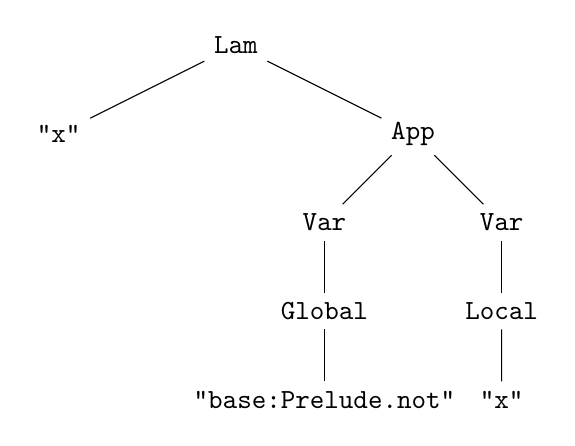
\begin{tikzpicture}[scale=0.75, level/.style={sibling distance=60mm/#1}]
      % Tree
      \node {\texttt{Lam}}
        child {node {\texttt{"x"}}}
        child {node {\texttt{App}}
          child {node {\texttt{Var}}
            child {node {\texttt{Global}}
              child {node {\texttt{"base:Prelude.not"}}}}}
          child {node {\texttt{Var}}
            child {node {\texttt{Local}}
              child {node {\texttt{"x"}}}}}};

      % Arrow
      %\node[single arrow,
      %      draw=black,
      %      fill=black!10,
      %      minimum height=2cm,
      %      shape border rotate=0] at (0,-1) {};
      %\draw[-latex] (A.east) -- (B.west);

      % Feature vector

  \end{tikzpicture}

  \caption{}

  \label{fig:featureextractionpic}
\end{figure}

\subsection{Clustering}
\label{sec:clustering}
% TODO
\fi

\section{Contributions}
\label{sec:contributions}

\subsection{Recurrent Clustering}
\label{sec:recurrentclustering}

We take the \emph{recurrent clustering} approach found in ML4PG and ACL2(ml), and implement a variant in the context of Haskell theory exploration. Here we give a brief description of recurrent clustering, describe our algorithm, and compare its similarity and differences to ML4PG and ACL2(ml).

\subsubsection{Overview}

\iffalse TODO: Much of this discussion reads as a minor implementation solution rather than an overview of the whole method \fi

\iffalse TODO: Focus the section more on the problem of identifiers, and how recurrent clustering uses clustering as part of feature extraction to solve this \fi

\iffalse TODO: Maybe present the translation from trees to matrices, to vectors first; leaving the conversion of terms to features until afterwards; similar to how ML4PG uses [foo] to mean ``the feature corresponding to foo, whatever that might be'' \fi

\iffalse TODO: Maybe present recurrent clustering in a ``naive'' way: define the conversion function ``[]'' recursively. Leave the dependency-ordering, etc. for the Algorithm section, as a way of ``building up to'' the result, which avoids the inefficiencies of recursing. \fi

The purpose of recurrent clustering, as with other clustering algorithms, is to identify similarities between a set of inputs. In our case, we want compare the abstract syntax trees of Core expressions, which presents a difficulty for clustering: many leaves are \emph{references}, containing identifiers for other expressions. For example, consider the following expressions which are identical except for an identifier:

\begin{equation*}
  \begin{split}
    X =\ & \texttt{App}\ (\texttt{Var}\ (\texttt{Local}\ \texttt{"f"}))\ (\texttt{Var}\ (\texttt{Global}\ \texttt{"odd"})) \\
    Y =\ & \texttt{App}\ (\texttt{Var}\ (\texttt{Local}\ \texttt{"f"}))\ (\texttt{Var}\ (\texttt{Global}\ \texttt{"even"})) \\
    Z =\ & \texttt{App}\ (\texttt{Var}\ (\texttt{Local}\ \texttt{"f"}))\ (\texttt{Var}\ (\texttt{Global}\ \texttt{"plus"}))
  \end{split}
\end{equation*}

Two possible methods for comparison are to ignore identifiers completely, or to compare them for equality. Neither is completely satisfactory, as the former will \emph{over-estimate} similarity (considering $X$, $Y$ and $Z$ to be the same), whilst the latter will \emph{under-estimate} similarity (considering $X$, $Y$ and $Z$ to be equidistant).

Ideally we would like something in between these two extremes, which requires a more sophisticated notion of similarity for identifiers. In the above example, we may intuitively consider \texttt{(\&\&)} and \texttt{(++)} to be closer to each other than to \texttt{map}; both in terms of \emph{definition} (e.g. only the former can be specified by pattern-matching on their first argument), and by their \emph{properties} (e.g. only the former can form monoids).

Recurrent clustering tackles this problem in a simple way: we look up the expressions \emph{referenced by} each identifier, and use \emph{their} similarity in place of the identifiers'. This gives rise to a recursive process, where feature extraction is interleaved with multiple rounds of clustering. For this recursive process to be well-founded, we impose a topological ordering on expressions based on their dependencies (the expressions they reference). This is slightly complicated in Haskell (compared to Coq, for example), since general recursion is permitted and several mutually-recursive expressions may appear at the same level.

\subsubsection{Algorithm}
\label{sec:algorithm}
\iffalse TODO: the code should go in the implementation section rather than here \fi
\iffalse TODO: give a more abstract presentation, using mathematical notation \fi
\iffalse TODO: maybe focus on the ``interesting cases'', and defer the nitty-gritty of extending the environment, etc. to the implementation section? \fi
\iffalse TODO: Define rose trees \fi
\iffalse TODO: Show an example from earlier, e.g. factorial \fi
\iffalse TODO: Split into three parts: expressions to rose trees of features; rose trees to matrices to vectors; k-means clustering \fi
\iffalse TODO: highlight the recurrent nature of the algorithm \fi
\iffalse TODO: I would probably just restructure:
 - start with the syntax, get to show how, for every line of figure 1, extraction works
 - then transformation to feature vectors
 - then k-means
obviously, they are mutually recursive...
\fi

Our algorithm proceeds in several stages. At the top level, we send named expressions to \hs{recurrentCluster}, topologically sorted: if an element contains multiple \hs{(Global, Expr)} pairs, they are mutually-recursive:

\begin{haskell}
recurrentCluster :: [[(Global, Expr)]] -> [[Global]]
recurrentCluster = go ([],[])
  where go (fs, db) []       = db
        go (fs, db) (es:ess) = let fs' = fs ++ map (extract db) es
                                   db' = kMeans fs'
                                in go (fs', db') ess
        extract db (i, e) = (i, rt db e)
\end{haskell}

The overall result of the \hs{recurrentCluster} function is a list of clusters, containing the IDs of their elements. These are obtained by interleaving clustering (the \hs{kMeans} function) and feature extraction (the \hs{rt} function).

The feature extraction itself contains two parts: first, syntax trees matching the grammar in figure \ref{fig:coresyntax} are converted into \hs{RoseTree}s with features (\hs{Float}s) on their \hs{Node}s:

\begin{haskell}
data RoseTree = Node Feature [RoseTree]

eRT :: [Local] -> [[Global]] -> Expr -> RoseTree
eRT env db e = case e of
  ...
\end{haskell}

The easiest branches to handle are literals and types, which we represent using particular feature values (\hs{sLITNUM}, \hs{sLITSTR} and \hs{sTYPE}):

\begin{haskell}
  Lit (LitNum _) -> Node sLITNUM []
  Lit (LitStr _) -> Node sLITSTR []
  Type           -> Node sTYPE   []
\end{haskell}

Function application simply recurses into both sub-expressions:

\begin{haskell}
  App e1 e2 -> Node sAPP [eRT env db e1,
                          eRT env db e2]
\end{haskell}

To look up variables locally and globally, we use the \hs{lookupL} and \hs{lookupG} functions, respectively. These return the index containing their argument, if found. In the case of \hs{lookupL}, this acts as a de Bruijn index to give alpha-equivalent terms equal feature vectors. For \hs{lookupG}, this is the ID of the cluster it appears in; this ensures that references to similar expressions result in similar features:

\begin{haskell}
  Var (Global i) -> Node (lookupG db  i) []
  Var (Local  i) -> Node (lookupL env i) []
\end{haskell}

Finally, when we traverse binders we must extend the environment \hs{env}:

\begin{haskell}
  Lam  i  e     -> Node sLAM [eRT (i:env) db e]
  Let  bs e     -> Node sLET (map (bRT (ids bs:env) db) bs ++
                                   eRT (ids bs:env) db  e
  Case e i alts -> Node sCASE (eRT    env  db  e :
                          map (aRT (i:env) db) alts)
\end{haskell}

Patterns and bindings are handled in a similar way:

\begin{haskell}
aRT :: [Local] -> [[Global]] -> Alt -> RoseTree
aRT env db alt = case alt of
  (DataAlt _, vs, e) -> eRT (vs ++ env) db e
  (LitAlt  _, _,  e) -> eRT env db e
  (Default,   _,  e) -> eRT env db e

bRT :: [Local] -> [[Global]] -> Bind -> RoseTree
bRT env db b = case b of
  NonRec i e -> eRT env db e
  Rec es     -> Node sREC (map (eRT env db . snd) es)
\end{haskell}

The result of \hs{eRT} is a \hs{RoseTree} whose branching structure mimics that of our original expression. We next need to convert this to a \emph{matrix} of features, which we do by converting each level of the \hs{RoseTree} into a row of the matrix (using \hs{pad} to ensure a consistent size). Finally we turn the matrix into a \emph{feature vector} by concatenating the rows:

\begin{haskell}
level :: Int -> RoseTree -> [Feature]
level 0 (Node x xs) = [x]
level n (Node x xs) = concatMap (level (n-1)) xs

rt :: [[Global]] -> Expr -> [Feature]
rt db e = concat (pad cols (map (`level` eRT [] db e) [0..rows]))
\end{haskell}

Notice that this algorithm contains several parameters, including \hs{rows} and \hs{cols} which determine how to truncate the matrices (defaults are 30). The \hs{kMeans} function also contains a parameter for the cluster number; we set this as $\sqrt{n}$ where $n$ is the number of feature vectors being clustered.

\subsubsection{Comparison}

Our algorithm is most similar to that of ML4PG, as our transformation maps each element in a tree to a distinct cell in its matrix. In contrast, the matrices produced by ACL2(ml) \emph{summarise} the tree elements: providing, for each level of the tree, the number of variables, nullary symbols, unary symbols, etc.

There are two major differences between our algorithm and that of ML4PG: mutual-recursion and types.

The special handling required for mutual recursion is discussed above (namely, topological sorting of expressions and the \hs{sUNKNOWN} sentinel). Such handling is not present in ML4PG, since the Coq code it analyses must, by virtue of the language, be written in dependency order to begin with. Coq \emph{does} have limited support for mutually-recursive functions, of the following form:

\begin{coqblock}
Fixpoint even n := match n with
                       | O   => true
                       | S m => odd m
                   end
    with odd  n := match n with
                       | O   => false
                       | S m => even m
                   end.
\end{coqblock}

However, this is relatively uncommon and unsupported by ML4PG.

The more interesting differences come from our handling (or lack thereof) for types. Coq and ACL2 are at opposite ends of the typing spectrum, with the former treating types as first class entities of the language whilst the latter is untyped (or \emph{unityped}). In both cases, we have a \emph{single} language to analyse, by ML4PG and ACL2(ml) respectively.\footnote{ML4PG can also analyse Coq's \textsc{Ltac} meta-language. Haskell has its own meta-language, Template Haskell, but here we only consider the regular Haskell which it generates.}

The situation is different for Haskell, where the type level is distinct from the value level, and there are strict rules for how they can influence each other. In particular, Haskell values can depend on types (via the type class mechanism) but types cannot depend on values.

In our initial approach, we restrict ourselves to the value level. This has several consequences:

\begin{itemize}
  \item Although they are values, we cannot distinguish between data constructors, other than using exact equality.
  \item Since Core uses a single \texttt{Lam} abstraction for both value- and type-level parameters, we cannot always distinguish between them. This can cause a function's Core arity to be greater than its Haskell arity.
\end{itemize}

There is certainly promise in including types in our analysis, by pairing every term with its type as in ML4PG. This will allow fine-grained distinction of expressions which are otherwise identical, especially data constructors.

\section{Implementation}
\label{sec:implementation}

We provide an implementation of our recurrent clustering algorithm in a tool called \textsc{ML4HS}, which consists of a loose collection of components shown in Figure \ref{fig:ml4hs}. This arrangement makes it easy to swap out parts for experimentation. In the following, we describe the custom components in the order they appear in the diagram.

\begin{figure}
  \centering
  \tikzstyle{block} = [rectangle, draw, rounded corners]
  \tikzstyle{container} = [rectangle, draw, rounded corners]
  \tikzstyle{line} = [draw, -latex']
  \colorlet{shade}{rgb:black,1;white,4}

  \begin{tikzpicture}[node distance=2cm]
    \node [block] (hackage) {Hackage};

    \node [block, below of=hackage] (cabal) {
      \begin{tikzpicture}[node distance = 2cm]
        \node (caballabel) {Cabal};
        \node [block, anchor=north west] at (caballabel.south) (ghc) {
          \begin{tikzpicture}[node distance = 2cm]
            \node (ghclabel) {GHC};
            \node [block, anchor=north west, fill=shade] at (ghclabel.south) (plugin) {AST Plugin};
          \end{tikzpicture}
        };
      \end{tikzpicture}
    };

    \node [block, below of=cabal, fill=shade]  (sorting) {Sorting};

    \node [block, below of=sorting, fill=shade] (clustering) {
      \begin{tikzpicture}[node distance = 2cm, auto]
        \node (clusterlabel) {Recurrent Clustering};
        \node [block, anchor=north west, fill=shade] at (clusterlabel.south west) (fe) {Feature Extraction};
        \node [block, anchor=west, fill=white] at ([xshift=2em]fe.east) (weka) {Weka};

        \path [line] (fe)   -- (weka);
        \path [line] (weka) -- (fe);
      \end{tikzpicture}
    };

    \node [block, below of=clustering, fill=shade] (mlspec) {
      \begin{tikzpicture}[node distance = 2cm, auto]
        \node (mlspeclabel) {MLSpec};
        \node [block, anchor=north west, fill=white] at (mlspeclabel.south) (qs) {QuickSpec};
      \end{tikzpicture}
    };

    \node [block, below of=mlspec] (user) {User};

    \path [line] (hackage)    -- (cabal);
    \path [line] (cabal)      -- (sorting);
    \path [line] (sorting)    -- (clustering);
    \path [line] (clustering) -- (mlspec);
    \path [line] (mlspec)     -- (user);
  \end{tikzpicture}
  \caption{Components of the ML4HS theory exploration system. Custom components are shaded, arrows indicate data flow.}
  \label{fig:ml4hs}
\end{figure}

\subsection{\textsc{AST Plugin}}
\label{sec:astplugin}

The GHC compiler provides mechanisms for parsing Haskell source code and converting it to Core. It also includes a \emph{renaming} transformation, which resolves global identifiers into a canonical form. This allows us to spot repeated use of a term, across multiple modules and packages, with a simple syntactic equality check.

Since we are interested in comparing definitions based on the terms they reference, building our framework on top of GHC seems like a promising approach. Indeed, \hspec{} already invokes GHC's API to obtain the definitions of Haskell functions, in order to transform them into a form suitable for ATP systems. However, our initial experiments showed that this technique is too fragile for use on many real Haskell projects.

This is due to many projects having a complex module structure, requiring particular GHC flags to be given, or using pre-processors such as \texttt{cpp} and Template Haskell to generate parts of their code. All of this complexity means that invoking GHC ``manually'' via its API is unlikely to obtain the definitions we require.

Thankfully there is one implementation detail which most Haskell packages agree on: the Cabal build system. All of the above complexities will be specified in a package's ``Cabal file'', such that the \texttt{cabal configure} and \texttt{cabal build} commands are very likely to work for most packages, without any extra effort. This shifted our focus to augmenting GHC and Cabal, such that definitions can be collected during the normal Haskell build process.

GHC provides a plugin mechanism for manipulating Core during a build, intended for optimisation passes, which we use to inspect definitions as they are being compiled. We provide a plugin called \textsc{AstPlugin} which emits a serialised version of each Core definition to the console (to satisfy the type system, it also implements a dummy ``optimisation'' which returns the Core unchanged).

Compared to Haskell, Core is a much simpler language and its representation is relatively stable compared to many existing representations of Haskell (which often change to support various language extensions). Three areas which make Core difficult to handle are:

\begin{description}
  \item{Type variables}: Parametric polymorphism (described in more detail in \S \ref{sec:haskelldesc}) can be thought of as values being parameterised by type-level objects. In System F, this is represented explicitly by a special abstraction form $\Lambda$, distinct from the $\lambda$ used for values. Core only has one abstraction form, \CLam, for both types and values. This alters function properties like arity.

  \item{Unified namespace}: Haskell has distinct namespaces for values, types, data constructors, etc. Since Core does not make these distinctions, names may become ambiguous. For example, a type parameter \hs{t} may be confused with a function argument \hs{t}. To prevent this, overlapping namespaces are distinguished by prefices which are distinct from the available names; for example a type class constraint \hs{Ord t} may give rise to a binder $\CLam\ \hs{"\$dOrd"}$ in Core, which is guaranteed not to conflict since this name would be invalid in Haskell. This causes difficulties when looking up names, as these prefixed forms do not easily map back to the Haskell source.

  \item{Violating encapsulation}: Although Haskell allows names to be \emph{private} to a module, when compiling Core we have full access to private definitions, as well as references to private names from within other definitions. Hence the definitions we receive from \textsc{AstPlugin} will include private values which we cannot import into a theory exploration tool.
\end{description}

In practice, we work around these issues with a post-processing stage: for each named definition appearing in the output of \textsc{AstPlugin}, we attempt to reference that name within the GHCi interpreter. Names with the above problems will cause an error, and are discarded.

The result of building a Haskell package with \textsc{AstPlugin} enabled is a database of Haskell definitions, similar in some respects to \textsc{Hoogle} \cite{mitchell2008hoogle}. Definitions are indexed by a combination of their package name, module name and binding name. The definitions themselves are s-expressions representing the Core AST, with non-local references replaced by a combination of package name, module name and binding name, which makes it trivial to look up references in the database. Each definition also has an associated arity and type, obtained during the post-processing step mentioned above.

\subsection{Toplogical Sorting}

As described in \S \ref{sec:symbolstofeatures}, we must topologically sort the output of \textsc{AstPlugin} in order for our recurrent clustering to be well-founded. Since our database keys (containing the package, module and binding names, as described above) match our representation of non-local references, it is simple to walk each syntax tree to obtain the set of references it makes. In addition, the resulting set of (identifier, list-of-referenced-identifiers) pairs exactly matches the (vertex, list-of-successor-vertices) format used to represent directed graphs by the popular \hs{containers} library which ships with GHC. This provides an implementation of topological sort for strongly connected components, which we use as-is. A simple shell script loops through these SCCs, invoking the recurrent clustering component for each and appending the resulting features and clusters to the database.

\subsection{Feature Extraction}

The implementation of our feature extraction algorithm is a rather direct translation of the description given in \S \ref{sec:contributions} into Haskell. We parse the s-expressions generated by \textsc{AstPlugin} into algebraic data types which correspond directly to the definitions in Figure \ref{fig:coresyntax}; this is routine, so we omit the details for brevity. Similarly, we can represent rose trees with a datatype corresponding to the definition given in \S \ref{sec:expressionstovectors}:

\begin{haskell}
data RoseTree = Node Feature [RoseTree]
\end{haskell}

For simplicity we use the representation \hs{Feature = Int}, as we do not have fractional values. Since we represent the symbols $expr$, $id$, etc. from Figure \ref{fig:coresyntax} using different datatypes, we cannot write one big definition of $toTree$ or $\phi$ which works on all tokens. Each case shown in Figure \ref{fig:totree} and equations \ref{eq:feature}, \ref{eq:localfeature} and \ref{eq:globalfeature} appears in the implementation, although they are spread across several functions.

To support looking up local identifiers, our implementation of $toTree$ takes a context as argument, extending it as required. As an example of the complexity this adds, here is the \CCase\ branch of $toTree$:

\begin{lstlisting}[language=Haskell, xleftmargin=0pt, xrightmargin=0pt]
toTree :: Context -> Expr -> RoseTree
toTree ctx x = case x of
  ...
  Case e l as -> Node fCase (toTree ctx e : map (toTreeAlt (l:ctx)) as)
  ...
\end{lstlisting}

Breaking this down we can see \hs{fCase} representing the value of $\feature{\CCase}$, and a list of sub-trees defined in parentheses. The first subtree is a straightforward recursive call in an unmodified context: \mbox{\hs{toTree ctx e}}. The rest of the list is formed by applying the function \mbox{\hs{toTreeAlt (l:ctx)}} to each element of the list \hs{as} of \CAlt\ clauses.

The \hs{toTreeAlt} function contains those cases of $toTree$ which handle symbols in $alt$. We prepend the identifier \hs{l} to the context, to get the extended context \hs{l:ctx}. This is because \hs{l} will be bound the value of \hs{e}, in order to avoid re-computing its value several times.

The other clauses are handled in a similar way. The trickiest is the \CLet\ clause, since the local identifiers aren't directly available; we must extract them from their \CRec, \CNonRec\ and \CBind\ wrappers first, which we do using helper functions.

As shown above, the values from equations \ref{eq:feature} are encoded directly in $toTree$. For $phi(l \in \mathcal{L})$ we use standard Haskell functions to look up the required indices in the context:

\begin{lstlisting}[language=Haskell, xleftmargin=0.1\textwidth, xrightmargin=0.1\textwidth]
phiL :: Context -> Local -> Feature
phiL ctx x = case elemIndex x ctx of
  Nothing -> error (concat ["Local '", show x,
                            "' not in context '",
                            show ctx, "'"])
  Just i  -> (2 * alpha) + i
\end{lstlisting}

As explained in \S \ref{sec:symbolstofeatures}, local identifiers should always exist in the context. If this precondition doesn't hold, we abort the program with an error rather than continuing.

Global identifiers are kept as-is until we have access to the clusters from the last iteration. This takes place outside Haskell, using the \hs{jq} data processing tool.

Our implementation of $level$ exactly matches equation \ref{eq:level}:

\begin{haskell}
level :: Int -> RoseTree -> [[Feature]]
level 1 (Node f _)  = [f]
level n (Node _ ts) = concatMap (level (n-1)) ts
\end{haskell}

To produce feature vectors, we do not directly construct the matrix; instead we generate the rows and concatenate them together in one step, using the \hs{concatMap} function:

\begin{lstlisting}[language=Haskell, xleftmargin=0.1\textwidth, xrightmargin=0.1\textwidth]
featureVec :: Expr -> [Feature]
featureVec e = concatMap (\m -> pad (level m tree)) [1..r]
  where tree   = toTree [] e
        pad xs = take c (xs ++ repeat 0)
\end{lstlisting}

By providing \hs{featureVec} with the latest set of clusters, read from the \textsc{AstPlugin} database, we turn Core expressions into feature vectors, which are appended to the database.

We use the Weka system to perform our k-means clustering, as it is widely used, including by ML4PG. We select all feature vectors from our database, and write them in CSV format for Weka to process. The Weka CLI command is invoked, which appends a cluster number to each of these feature vectors; we read these off and append them to the database. As long as more SCCs remain unprocessed, we keep looping this process, using the database to communicate between the feature extraction and clustering phases.

\subsection{\textsc{MLSpec}}
\label{sec:mlspec}

We cannot supply these clusters as-is to \qspec{}, since it must be provided with a \emph{signature}. These are constructed by our \textsc{MLSpec} tool, using information from the \textsc{AstPlugin} database. Tasks performed by \textsc{MLSpec} include:

\begin{itemize}
  \item{Monomorphising}: Given values of polymorphic type, e.g. \hs{safeHead :: forall t. [t] -> Maybe t} and \hs{[] :: forall t. [t]}, a testing-based system like \qspec{} is unable to evaluate these expressions without instantiating the variable \hs{t} to a specific type. Such an instantiation is called \emph{monomorphising}, and in the case of \textsc{MLSpec} we build on previous work in \qcheck{} by attempting to instantiate all type variables to \hs{Integer}. We discard those cases where this is invalid, such as variable \emph{type constructors} (e.g. \hs{forall c. c Bool -> c Bool}) or incompatible class constraints (e.g. \hs{forall t. IsString t => t}).

  \item{Qualification}: All names are \emph{qualified} (prefixed by their module's name), to avoid most ambiguity. There is still the possibility that multiple packages will declare modules of the same name, although this is rare as it causes problems for any Haskell programmer trying to use those modules. In such cases the exploration process simply aborts.

  \item{Variable definition}: Once a \qspec{} theory has been defined containing all of the given terms, we inspect the types it references and append three variables for each to the theory (enough to discover laws such as associativity, but not too many to overflow the limit of \qspec{}'s exhaustive search).

  \item{Sandboxing}: One difficulty with Haskell's packaging infrastructure is that all required packages and modules must be provided up-front, usually by specification in a Cabal file. Since \textsc{MLSpec} builds signatures \emph{dynamically}, depending on the cluster information it is given, we do not know what packages it may need. To work around this problem, \textsc{MLSpec} invokes \qspec{} for each cluster using a library we have built called \texttt{nix-eval}. This provides an \texttt{eval} function, like those commonly found in dynamic languages such as Python and Javascript, for evaluating Haskell expressions. The key feature of \texttt{nix-eval} is that these Haskell expressions may reference packages that are not installed on the system. When such expressions are evaluated, these packages will be automatically downloaded and installed into a sandbox using the Nix package manager, and GHC will be invoked in this sandbox to perform the evaluation.

\end{itemize}


\iffalse
\section{First Results}

TODO

Future work?
Hypothetical use cases?
\fi

\section{Related Work}
\label{related}

\subsection{Haskell}
\label{haskelldesc}

Haskell is a convenient choice for our purposes for several reasons. Here we discuss the relevant language features from a high-level:

\begin{description}

\item{Functional}: All control flow is performed by function abstraction and application, which we can reason about using standard rules of inference such as \emph{modus ponens}.

\item{Pure}: Execution of actions (e.g. reading files) is separate to evaluation of expressions; hence our reasoning can safely ignore complicated external and non-local interactions.

\item{Statically Typed}: Expression are constrained by \emph{types}, which can be used to eliminate unwanted combinations of values, and hence reduce search spaces; \emph{static} types can be deduced syntactically, without having to execute the code.

\item{Non-strict}: If an evaluation strategy exists for $\beta$-normalising an expression (i.e. performing function calls) without diverging, then a non-strict evaluation strategy will not diverge when evaluating that expression. This is rather technical, but in simple terms it allows us to reason effectively about a Turing-complete language, where evaluation may not terminate. For example, when reasoning about \emph{pairs} of values \hs{(x, y)} and projection functions \hs{fst} and \hs{snd}, we might want to use an ``obvious'' rule such as $\forall \text{\hs{x y}}, \text{\hs{x}} = \text{\hs{fst (x, y)}}$. Haskell's non-strict semantics makes this equation valid; whilst it would \emph{not} be valid in the strict setting common to most other languages, where the expression \hs{fst (x, y)} will diverge if \hs{y} diverges (and hence alter the semantics, if \hs{x} doesn't diverge).

\item{Algebraic Data Types}: These provide a rich grammar for building up user-defined data representations, and an inverse mechanism to inspect these data by \emph{pattern-matching}. For our purposes, the useful consequences of ADTs and pattern-matching include their amenability for inductive proofs and the fact they are \emph{closed}; i.e. an ADT's declaration specifies all of the normal forms for that type. This makes exhaustive case analysis trivial, which would be impossible for \emph{open} types (for example, consider classes in an object oriented language, where new subclasses can be introduced at any time).

\item{Parametricity}: This allows Haskell \emph{values} to be parameterised over \emph{type-level} objects; provided those objects are never inspected. This has the \emph{practical} benefit of enabling \emph{polymorphism}: for example, we can write a polymorphic identity function \hs{id :: forall t. t -> t}. \footnote{Read ``\hs{a :: b}'' as ``\hs{a} has type \hs{b}'' and ``\hs{a -> b}'' as ``the type of functions from \hs{a} to \hs{b}''.} Conceptually, this function takes \emph{two} parameters: a type \hs{t} \emph{and} a value of type \hs{t}; yet only the latter is available in the function body, e.g. \hs{id x = x}. This inability to inspect type-level arguments gives us the \emph{theoretical} benefit of being able to characterise the behaviour of polymorphic functions from their type alone, a technique known as \emph{theorems for free} \citep{wadler1989theorems}.

\item{Type classes}: Along with their various extensions, type classes are interfaces which specify a set of operations over a type (or other type-level object, such as a \emph{type constructor}). Many type classes also specify a set of \emph{laws} which their operations should obey but, lacking a simple mechanism to enforce this, laws are usually considered as documentation. As a simple example, we can define a type class \hs{Semigroup} with the following operation and associativity law:

\begin{lstlisting}[language=Haskell, xleftmargin=.2\textwidth, xrightmargin=.2\textwidth]
op :: forall t. Semigroup t => t -> t -> t
\end{lstlisting}

$$\forall \text{\hs{x y z}}, \text{\hs{op x (op y z)}} = \text{\hs{op (op x y) z}}$$

The notation \hs{Semigroup t =>} is a \emph{type class constraint}, which restricts the possible types \hs{t} to only those which implement \hs{Semigroup}. \footnote{Alternatively, we can consider \hs{Semigroup t} as the type of ``implementations of \hs{Semigroup} for \hs{t}'', in which case \hs{=>} has a similar role to \hs{->} and we can consider \hs{op} to take \emph{four} parameters: a type \hs{t}, an implementation of \hs{Semigroup t} and two values of type \hs{t}. As with parameteric polymorphism, this extra \hs{Semigroup t} parameter is not available at the value level. Even if it were, we could not alter our behaviour by inspecting it, since Haskell only allows types to implement each type class in at most one way, so there would be no information to branch on.} There are many \emph{instances} of \hs{Semigroup} (types which may be substituted for \hs{t}), e.g. \hs{Integer} with \hs{op} performing addition. Many more examples can be found in the \emph{typeclassopedia} \citep{yorgey2009typeclassopedia}. This ability to constrain types, and the existence of laws, helps us reason about code generically, rather than repeating the same arguments for each particular pair of \hs{t} and \hs{op}.

\item{Equational}: Haskell uses equations at the value level, for definitions; at the type level, for coercions; at the documentation level, for typeclass laws; and at the compiler level, for ad-hoc rewrite rules. This provides us with many \emph{sources} of equations, as well as many possible \emph{uses} for any equations we might discover. Along with their support in existing tools such as SMT solvers, this makes equational conjectures a natural target for our investigation.

\item{Modularity}: Haskell has a module system, where each module may specify an \emph{export list} containing the names which should be made available for other modules to import. When such a list is given, any expressions \emph{not} on the list are considered \emph{private} to that module, and are hence inaccessible from elsewhere. This mechanism allows modules to provide more guarantees than are available just in their types. For example, a module may represent email addresses in the following way:

\begin{lstlisting}[language=Haskell, xleftmargin=.2\textwidth, xrightmargin=.2\textwidth, upquote=true]
module Email (Email(), at, render) where

data Email = E String String

render :: Email -> String
render (E u h) = u ++ "@" ++ h

at :: String -> String -> Maybe Email
at "" h  = Nothing
at u  "" = Nothing
at u  h  = Just (E u h)
\end{lstlisting}

The \hs{Email} type guarantees that its elements have both a user part and a host part (modulo divergence), but it does not provide any guarantees about those parts. We also define the \hs{at} function, a so-called ``smart constructor'', which has the additional guarantee that the \hs{Email}s it returns contain non-empty \hs{String}s. By ommitting the \hs{E} constructor from the export list on the first line \footnote{The syntax \hs{Email()} means we're exporting the \hs{Email} type, but not any of its constructors.}, the only way \emph{other} modules can create an \hs{Email} is by using \hs{at}, which forces the non-empty guarantee to hold globally.

\end{description}

Together, these features make Haskell code highly structured, amenable to logical analysis and subject to many algebraic laws. However, as mentioned with regards to type classes, Haskell itself is incapable of expressing or enforcing these laws (at least, without difficulty \citep{lindley2014hasochism}). This reduces the incentive to manually discover, state and prove theorems about Haskell code, e.g. in the style of interactive theorem proving (see \S \ref{itp}), as these results may be invalidated by seemingly innocuous code changes. We will revisit the second-class status of theorem proving in Haskell in our discussion of theory exploration (\S \ref{theoryexploration}), but we will remark that Haskell is thus in a unique position with regards to the discovery of interesting theorems. Namely that many discoveries may be available with very little work, simply because the code's authors are focused on \emph{software} development rather than \emph{proof} development. The same cannot be said, for example, of ITP systems; although our reasoning capabilities may be stronger in an ITP setting, much of the ``low hanging fruit'' will have already been found through the user's dedicated efforts, and hence TE would be more likely to fit into an automation role for the user, rather than providing truly unexpected new discoveries.

Other empirical advantages to studying Haskell, compared to either other programming languages or theorem proving systems, include:

\begin{itemize}

\item The large amount of Haskell code which is freely available online, e.g. in repositories like \href{http://hackage.haskell.org}{Hackage}, with which we can experiment.

\item The existence of conjecture generation and theory exploration systems for Haskell, such as \qspec{} and \hspec{}, and counterexample finders like \qcheck{}, \textsc{SmallCheck} and \textsc{SmartCheck}.

\item The remarkable amount of infrastructure which exists for working with Haskell code, including package managers, compilers, interpreters, parsers, static analysers, etc.

\end{itemize}

\iffalse

\subsection{Conjecture Generation}

The task of \emph{conjecture generation} lies at the heart of theory exploration, and

\subsubsection{Lemma generation}

\fi

\subsection{Exploration in Artificial Intelligence}

Theorem proving is not the only area of AI to have automation extended from problem \emph{solving} to problem \emph{invention}. Here we consider similar approaches in a variety of domains, and identify techniques which could be re-purposed in the context of theory exploration.

\subsubsection{Evolutionary Computation}

\emph{Evolutionary computation} is an umbrella term for heuristic search algorithms which mimic the process of evolution by natural selection among a population of candidate solutions \citep{back1997evolutionary}. Whilst \emph{genetic algorithms} are perhaps the most well-known instance of evolutionary computation, their use of \emph{strings} to represent solutions causes complications when comparing to a domain like theory exploration, where recursive structures of unbounded depth arise. Thankfully these problems are not insurmountable, for example \emph{genetic programming} can operate on tree-structures natively \citep{banzhaf1998genetic}, which makes evolutionary computation a useful source of ideas for reuse in our theory exploration setting.

Traditionally, evolutionary approaches assign solutions a \emph{fitness} value, using a user-supplied \emph{fitness function}. Fitness should correlate with how well a solution solves the user's problem; for example, the fitness of a solution to some engineering problem may depend on the estimated materials cost. If we frame the task of theory exploration in evolutionary computation terms, the fitness function would be our interestingness measure.

Pure exploration (i.e. for its own sake) has been studied in evolutionary computation for two main reasons: \emph{artificial life} and \emph{deceptive problems}. The former attempts to gain insight into the nature of life and biology through competition over limited resources. Whilst this may have utility in resource allocation, e.g. efficient scheduling of a portfolio of ATP programs, there is no direct connection to interestingness in theory exploration, so we will not consider it further (note that similar resource-usage ideas can also be found in the literature on \emph{artificial economies}, e.g. \citep{baum2000evolution}).

On the other hand, work on deceptive problems is highly relevant, as it has lead to studying various notions of intrinsic fitness, which are analogous to the interestingness measures we want. Deceptive problems are those where \textquote{pursuing the objective may prevent the objective from being reached} \citep{lehman2011abandoning}, which is caused by the fitness (objective) function having many local optima which are easy to find (e.g. by hill climbing), but few global optima which are hard to find. Many approaches try to avoid deception by augmenting the given fitness function to promote \emph{diversity} and \emph{novelty}, such as \emph{niching methods} \citep{sareni1998fitness}.

One example is \emph{fitness sharing}, which divides up fitness values between identical or similar solutions. Say we have a user-provided fitness function $f$, and a population containing two identical solutions $s_1$ and $s_2$; hence $f(s_1) = f(s_2)$. In a fitness sharing scheme, we interpret fitness as a fixed resource, distributed according to $f$; when multiple individuals occupy the same point in the solution space, they must \emph{share} the fitness available there. We can describe the fitness \emph{allocated} to a solution by augmenting $f$, e.g. if we allocate fitness uniformly between identical solutions we get:

$$f'(x) = \frac{f(x)}{\sum_{i=1}^n \delta_{s_i x}}$$

Where $n$ is the population size, $s_i$ is the $i$th solution in the population and $\delta$ is the Kronecker delta function. In the example above, assuming there are no other copies in the population, then $f'(s_1) = \frac{f(s_1)}{2} = \frac{f(s_2)}{2} = f'(s_2)$. By sharing in this way, the fitness of each solution is balanced against redundancy in the population: there may still be many copies of a solution, but only when the fitness is high enough to justify all of them.

There are many variations on this theme, such as sharing between ``close'' solutions rather than just identical ones and judging distance based on fitness (AKA phenotypically) rather than based on the location in solution space (AKA genetically). Yet the underlying principle is always the same: penalise duplication in order to promote diversity. This lesson can be carried over to our theory exploration context, where a theorem should be considered less interesting if it is ``close'' to others which have been found.

In a similar way, we can bias our search procedure, rather than our fitness function, towards diversity. The search procedure in population-based evolutionary algorithms consists of \emph{selecting} one or more individuals from the population, e.g. via truncation (select the best $n$ individuals, discarding the rest); then \emph{transforming} the selected individuals, e.g. via mutation and crossover, to obtain new solutions.

\newcommand{\argmin}{\operatornamewithlimits{argmin}}

Traditional selection methods are biased towards high fitness individuals (this is especially clear for truncation). Alternative schemes have been proposed which favour diversity \emph{at the expense of} fitness. For example, the fitness uniform selection scheme (FUSS) \citep{hutter2002fitness} selects a target fitness $f_t$ uniformly from the interval $\left[ f_{min}, f_{max} \right]$ between the highest and lowest of the population. An individual $s$ is then selected with fitness closest to $f_t$, i.e. $s = \operatornamewithlimits{argmin}\limits_{x} \lvert f(x) - f_t \rvert$

In this way, the fitness function $f$ is used to assign comparable quantities to solutions, but it is not treated as the objective; instead, the implicit objective is to maintain a diverse population, with individuals spread out uniformly in fitness space. This approach seems useful for informing our work in theory exploration, as it supports search criteria which \emph{describe} solutions, but which we may not want to \emph{optimise}. As a simple example, we might distinguish different forms of theorem by measuring how balanced their syntax trees are (-1 for left-leaning, +1 for right leaning, 0 for balanced); but it would be senseless to \emph{maximise} how far they lean.

Once we begin this process of augmenting fitness functions, or abandoning their use as objectives, an obvious question arises: what happens if our new function contains nothing of the original? This kind of pure exploration scenario leads to a variety of ideas for \emph{instrinsic} fitness, such as novelty \citep{lehman2011abandoning}, which can lead to learning useful ``stepping stones'' even in objective-driven domains. Such intrinsic notions of fitness are direct analogues of the interestingness measures we seek for theory exploration.

\subsubsection{Artificial Curiosity}
\label{curiosity}

\begin{figure}
  \centering
  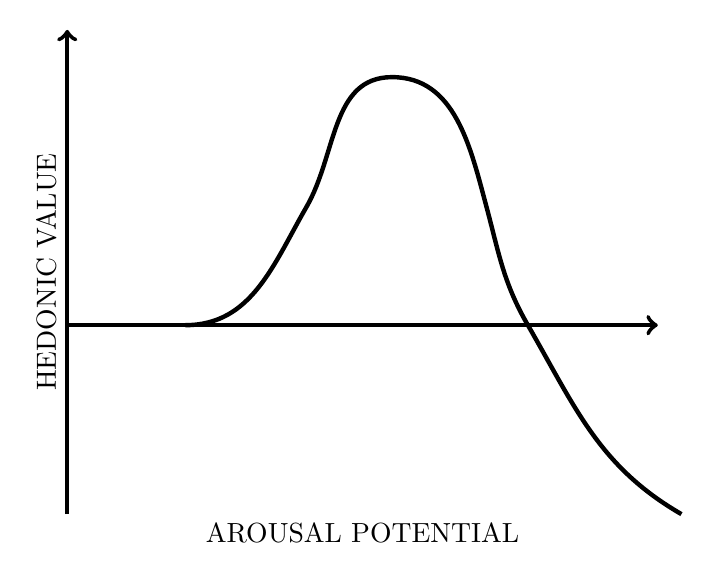
\begin{tikzpicture}[scale=0.75]
      % The image, for reference
      % \node[anchor=south west,inner sep=0] at (0,0) {\includegraphics[width=\textwidth]{wundt.png}};

      % Axes
      \draw[black,ultra thick,->] (1,0.8) -- (1,  9)   node[midway, above, sloped] {HEDONIC VALUE};     % y axis
      \draw[black,ultra thick,->] (1,4)   -- (11, 4);                                                   % x axis
      \path                       (1,0.8) -- (11, 0.8) node[midway, below]         {AROUSAL POTENTIAL}; % x axis label

      % Curve. The numbers come from tracing over wundt.png
      \draw[black,ultra thick] (3, 4)
           to[out=0,   in=240] (5.05, 6)
           to[out=60,  in=180] (6.5,  8.2)
           to[out=0,   in=105] (8.1,  6)
           to[out=-75, in=120] (8.8,  4)
           to[out=-60, in=150] (11.4, 0.8);

      % This version is closer, but a little jagged
      \iffalse
      \draw[black,ultra thick] (3, 4)
           to[out=0,   in=240] (5.05, 6)
           to[out=60,  in=225] (6,    8)
           to[out=45,  in=180] (6.5,  8.2)
           to[out=0,   in=135] (7.2,  8)
           to[out=-45, in=105] (8.1,  6)
           to[out=-75, in=120] (8.8,  4)
           to[out=-60, in=150] (11.4, 0.8);
      \fi
  \end{tikzpicture}

  \caption{The Wundt curve, reproduced from \citep{berlyne1970novelty}. The axes ``hedonic value'' and ``arousal potential'' are described as covering \textquote{reward value\dots preference or pleasure}, and \textquote{all the stimulus properties that tend to raise arousal, including novelty and complexity}, respectively.}

  \label{wundt}
\end{figure}

\emph{Artificial curiosity} (AC) describes active learning systems which are rewarded based on how interesting the input or data they discover is \citep{schmidhuber2006developmental}. Although framed in the context of \emph{reinforcement learning}, this is clearly relevant to our theory exploration setting.

As an unsupervised learning task, AC has no access to labels or meanings associated with its input; the only features it can learn are the structure and relationships inherent in the data, which is very much what we would like a theory exploration system to do. The unifying principle of AC methods is to force systems away from inputs which are not amenable to learning; either because they are so familiar that there is nothing left to learn, or so unfamiliar that they are unintelligible. The resulting behaviour is characterised by the \emph{Wundt curve} (shown in figure \ref{wundt}) \footnote{In practice, many measures avoid negative values for simplicity, in which cases we replace all negative points on the curve with zero.}, which has been used in psychology to explain human aesthetics and preferences \citep{berlyne1970novelty}.

We can divide AC approaches into two groups: the first, which we call \emph{explicit}, send inputs which follow a Wundt curve to their learning algorithm; the second, the \emph{implicit} approaches, instead modify the \emph{output} of their learning algorithm(s), such that the overall system follows a Wundt curve as an emergent property.

In the explicit case, the \emph{implicit reward} signals being learned are analogous to our notion of interestingness. A framework encompassing many examples is given in \citep{oudeyer2007intrinsic} in the context of reinforcement learning.

One particularly general measure is \emph{compression progress}: given a compressed representation of our previous observations, the ``progress'' is the space saved if we include the current observation. Observations which are incompressible or trivially compressible don't save any space, whilst observations which provide new information relevant to past experience can provide a saving. This can be translated to a theorem proving context very naturally: our observations are theorems and their proofs, whilst new theorems which generalise known results will allow us to compress their proofs.

% TODO: Examples
\citep{Schmidhuber1999}

Two sources of intrinsic reward are proposed in \citep{Hester.Stone:2012} for \emph{random forests}. A random forest is a population of decision trees, where each tree is trained on a sub-set of the available examples, each decision is made using a sub-set of the available features, and the predictions of every tree are averaged to obtain that of the forest \citep{randomforests}. The first intrinsic reward is the \emph{disagreement} between predictions; for a forest with $m$ models (trees), predicting features $x_1$ \dots $x_n$ of the state resulting from taking action $a$ in state $s$, we simply sum the Kullback-Leibler divergence $D_{\rm KL}$ of each prediction $P_1$ \dots $P_m$ from every other prediction:

\begin{equation}
  D(s,a) = \sum_{i = 1}^n \sum_{j = 1}^m \sum_{k = 1}^m D_{KL}(P_j(x_i|s,a) || P_k(x_i|s,a))
\end{equation}

$D(s,a)$ is an explicit AC reward, as it follows a Wundt curve as the complexity of transitions increases. For parts of the state space which have been fully learned, the models will agree on accurate predictions. For parts which are unlearnable, the models cannot infer any structure, and will converge to reporting the average of past observations; these predictions may not be accurate, but they will be in agreement. Hence it is the states which are amenable to learning which produce the largest disagreement.

The second intrinsic reward is simply a measure of distance from previous observations, which pushes the system towards unseen states regardless of how learnable they are (similar to the $R_{max}$ technique). This is too simple to meet our definition of AC, but it does force the models to generalise their predictions to unexplored states, acting to increase disagreement in the forest.

A key advantage of random forests is that their models are \emph{inspectable}: they not only give predictions, but also \emph{reasons} for those predictions (i.e. we can see which paths are taken through each decision tree). % TODO: The accuracy of these random forest models are compared

% TODO
\citep{Kaplan2006}
\citep{Lipson2007}
\citep{Luciw2011}
\citep{Macedo2000}
\citep{Ramik.Sabourin.Madani:2013}
\citep{Roa.Kruijff.Jacobsson:2009}
\citep{Schaul.Sun.Wierstra.ea:2011}
\citep{Schmidhuber1999}
\citep{Schmidhuber:1991}
\citep{Scott1989}
\citep{Steunebrink.Koutnik.Thorisson.ea:2013}
\citep{maher2008achieving}
\citep{meyer1991possibility}
\citep{oudeyer2004intelligent}
\citep{oudeyer2014evolution}
\citep{schmidhuber2006developmental}

% TODO: Coevolution

Whilst clearly of relevance to theory exploration, artificial curiosity is usually framed in the context of a \emph{reinforcement learning} and \emph{intrinsic reward}, especially in the field of developmental robotics. This requires non-trivial choices to be made in deciding which of its concepts are of relevance to our domain, and how they may be translated across. For example, much of developmental robotics studies continuous, real-valued sensorimotor signals which may not have any direct analogue in the manipulation of logical formulae. However, if we take a higher-level view, the study of such signals may provide insight for predicting and tuning the behaviour of off-the-shelf ATP algorithms.

The most obvious contrast between developmental robotics and theory exploration is that the latter is not physically embodied (e.g. in a robot). Embodiment has been proposed as a necessary property of intelligent systems, as it provides \emph{grounding} \citep{anderson2003embodied}. Embodiment emerged as a response to the symbolic techniques of GOFAI, and in this sense the fields of theory exploration and developmental robotics seem incompatible. Nevertheless, TE can be seen to avoid the problems of GOFAI in two ways:

\begin{itemize}

  \item Firstly, the abstract, mathematical domain being explored is not a \emph{model} of some external, physical environment; the domain \emph{is} our environment; hence there is no issue of grounding terms with some external meaning.

  \item Secondly, there is a physical aspect of TE in that \emph{resource usage} is a critical factor. If it weren't, then brute force enumeration of proofs would be a viable solution. In this sense, we can provide physical inputs to our algorithms, such as measures of time and space used.

\end{itemize}

\iffalse

\subsubsection{Universal Drives}

PhysRevLett.110.168702.pdf
Omohundro? Too physical.
\emph{Universal drives} are those

\fi

\subsection{Statistics of Formal Systems}

The core problem of assigning ``interestingness'' to logical formulae is the application of statistical reasoning to the discrete, semantically-rich domain of formal systems. This problem has been tackled from various directions for a variety of reasons; here we summarise those contributions which seem of particular importance for theory exploration.

\subsubsection{Relevance Filtering}
\label{relevance}

% TODO
\citep{kuhlwein2012overview}

The combinatorial nature of formal systems causes many proof search methods, such as resolution, to have exponential complexity \citep{haken1985intractability}; hence even a modest size increase can turn a trivial problem into an intractable one. Finding efficient alternatives for such algorithms, especially those which are NP-complete (e.g. determining satisfiability) or co-NP-complete (e.g. determining tautologies), seems unlikely, as it would imply progress on the famously intractable open problems of $\text{P} = \text{NP}$ and $\text{NP} = \text{co-NP}$. On the other hand, we can turn this difficulty around: a modest \emph{decrease} in size may turn an intractable problem into a solvable one. We can ensure that the solutions to these reduced problems coincide with the original if we only remove \emph{redundant} information. This leads to the idea of \emph{relevance filtering}.

Relevance filtering simplifies a proof search problem by removing from consideration those clauses (axioms, definitions, lemmas, etc.) which are deemed \emph{irrelevant}. The technique is used in Sledgehammer during its translation of Isabelle/HOL theories to statements in first order logic: rather than translating the entire theory, only a sub-set of relevant clauses are included. This reduces the size of the problem and speeds up the proof search, but it creates the new problem of determining when a clause is relevant: how do we know what will be required, before we have the proof?

The initial approach, known as \textsc{MePO} (from \emph{Meng-Paulson} \citep{meng2009lightweight}), gives each clause a score based on the proportion $m / n$ of its symbols which are ``relevant'' (where $n$ is the number of symbols in the clause and $m$ is the number which are relevant). Initially, the relevant symbols are those which occur in the goal, but whenever a clause is found which scores more than a particular threshold, all of its symbols are then also considered relevant. There are other heuristics applied too, such as increasing the score of user-provided facts (e.g. given by keywords like \texttt{using}), locally-scoped facts, first-order facts and rarely-occuring facts. To choose $r$ relevant clauses for an ATP invocation, we simply order the clauses by decreasing score and take the first $r$ of them.

Recently, a variety of alternative algorithms have also been investigated, including:

\begin{description}

  \item{\textsc{MaSH}}: Machine Learning for SledgeHammer \citep{kuhlwein2013mash}. The distinguishing feature of \textsc{MaSH} is its use of ``visibility'', which is essentially a dependency graph of which theorems were used in the proofs of which other theorems; although theorems are represented as abstract sets of features. To select relevant clauses for a goal, the set of clauses which are visible from the goal's components is generated; this is further reduced by (an efficient approximation of) a naive Bayes algorithm.

  \item{\textsc{MOR}}: \emph{Multi-output ranking} uses a support vector machine (SVM) approach for selecting relevant axioms from the Mizar Mathematical Library for use by the Vampire ATP system \citep{alama2014premise}. \iffalse TODO: describe the kernel, as that's the interesting bit \fi It compares favourably to \textsc{SNoW} and \textsc{SInE}.

  % TODO:
  \item{\textsc{SInE}}
  \item{\textsc{BliStr}}
  \item{\textsc{HOLyHammer}}
  \item{\textsc{MoMM}}
  \item{\textsc{SNoW}}
  \item{\textsc{MPTP 0.2}}
  \item{\textsc{MaLARea}}
  \item{\textsc{MaLARea SG1}}

\end{description}

\subsubsection{Clustering}
\label{clustering}

% TODO: ML4PG
\citep{journals/corr/abs-1212-3618}
% TODO: ACL2(ml) (also examples section)
\citep{heras2013proof}

\subsubsection{Probability of Sentences}

The most important property of a logical formula is its truth value. Although we may be able to determine some truth values exactly, e.g. using decision or semi-decision procedures, it may be more efficient to \emph{approximate} truth values. One straightforward extension of truth values is \emph{probabilities}, where we can assign probability $1$ to formulae which are known to be true, $0$ to formulae known to be false, and intermediate values to those which we do not yet know.

% TODO
\citep{Hutter.Lloyd.Ng.ea:2013}

\subsubsection{Interestingness in Concept Formation}
\label{conceptformation}

% TODO:
\citep{Montano-Rivas.McCasland.Dixon.ea:2012}
\citep{Piantadosi.Tenenbaum.Goodman:2012}
\citep{Wille:2005}
\citep{colton1999automatic}
\citep{colton2000agent}
\citep{colton2012automated}
\citep{lenat1977automated}
\citep{mullerunderstanding}
\citep{Bundy.Cavallo.Dixon.ea:2015}
\citep{johansson2009isacosy}
\citep{spector2008genetic}
\citep{colton2012automated}
 \citep{geng2006interestingness}
% TODO: How does https en.wikipedia.org/wiki/Discovery system relate?

% However, this search space grows exponentially in the length of the proofs, which is unfortunate since proof length has been proposed as an approximate measure of how interesting a theorem is \cite[\S~10.2.1]{colton2012automated}.

% Alan Bundy et al

% Eurisko, AM, etc.?

\subsubsection{Learning From Structured Data}

One major difficulty with formal mathematics as a domain in which to apply statistical machine learning is the use of \emph{structure} to encode information in objects. In particular, \emph{trees} appear in many places: from inductive datatypes, to recursive function definitions; from theorem statements, to proof objects. Such nested structures may extend to arbitrary depth, which makes them difficult to represent with a fixed number of features, as is expected by most machine learning algorithms. Here we review a selection of solutions to this problem, and compare their distinguishing properties.


\paragraph{Truncation and Padding}

The simplest way to limit the size of our inputs is to truncate anything larger than a particular size (and pad anything smaller). This is the approach taken by ML4PG \citep{journals/corr/abs-1302-6421}, which limits itself to trees with at most 10 levels and 10 elements per level; each tree is converted to a $30 \times 10$ matrix (3 values per tree node) and learning takes place on these normalised representations.

Truncation is unsatisfactory in the way it balances \emph{data} efficiency with \emph{time} efficiency. Specifically, truncation works best when the input data contains no redundancy and is arranged with the most significant data first (in a sense, it is ``big-endian''). The less these assumptions hold, the less we can truncate. Since many ML algorithms scale poorly with input size, we would prefer to eliminate the redundancy using a more aggressive algorithm, to keep the resulting feature size as low as possible.

\paragraph{Dimension Reduction}

A more sophisticated approach to the problem of reducing input size is to view it as a \emph{dimension reduction} technique: our inputs can be modelled as points in high-dimensional spaces, which we want to project into a lower-dimensional space ($\left\{ {0, 1} \right\}^N$ in the case of $N$-bit vectors).

Truncation is a trivial dimension reduction technique: take the first $N$ coordinates (bits). More sophisticated projection functions consider the \emph{distribution} of the points, and project with the hyperplane which preserves as much of the variance as possible (or, equivalently, reduces the \emph{mutual information} between the points).

There are many techniques to find these hyperplanes, such as \emph{principle component analysis} (PCA) and \emph{autoencoding}; however, since these techniques are effectively ML algorithms in their own right, they suffer some of the same constraints we're trying to avoid:

\begin{itemize}
  \item They operate \emph{offline}, requiring all input points up-front
  \item All input points must have the same dimensionality
\end{itemize}

In particular, the second constraint is precisely what we're trying to avoid. Sophisticated dimension reduction is still useful for \emph{compressing} large, redundant features into smaller, information-dense representations, and as such provides a good complement to truncation.

The requirement for offline ``batch'' processing is more difficult to overcome, since any learning we perform for feature extraction will interfere with the core learning algorithm that's consuming these features (this is why deep learning is often done greedily).

\paragraph{Sequencing}

The task of dimension reduction changes when we consider \emph{structured} data. Recursive structures, like trees and lists, have \emph{fractal} dimension: adding layers to a recursive structure gives us more \emph{fine-grained} features, rather than \emph{orthogonal} features. For data mining context-free languages (e.g. those of programming and theorem-proving systems), we will mainly be concerned with tree structures of variable size.

Any investigation of variable-size input would be incomplete without mentioning \emph{sequencing}. This is a lossless approach, which splits the input into fixed-size \emph{chunks}, which are fed into an appropriate ML algorithm one at a time. The sequence is terminated by a sentinel; an ``end-of-sequence'' marker which, by construction, is distinguishable from the data chunks. This technique allows us to trade \emph{space} (the size of our input) for \emph{time} (the number of chunks in a sequence).

Not all ML algorithms can be adapted to accept sequences. One notable approach is to use \emph{recurrent ANNs} (RANNs), which allow arbitrary connections between nodes, including cycles. Compared to \emph{feed-forward} ANNs (FFANNs), which are acyclic, the \emph{future output} of a RANN may depend arbitrarily on its \emph{past inputs} (in fact, RANNs are universal computers).

The main problem with RANNs, compared to the more widely-used FFANNs, is the difficulty of training them. If we extend the standard backpropagation algorithm to handle cycles, we get the \emph{backpropagation through time} algorithm \citep{werbos1990backpropagation}. However, this suffers a problem known as the \emph{vanishing gradient}: error values decay exponentially as they propagate back through the cycles, which prevents effective learning of delayed dependencies, undermining the main advantage of RANNs. The vanishing gradient problem is the subject of current research, with countermeasures including \emph{neuroevolution} (using evolutionary computation techniques to train an ANN) and \emph{long short-term memory} (LSTM; introducing a few special, untrainable nodes to persist values for long time periods \citep{hochreiter1997long}).

The application of \emph{kernel methods} to structured information is discussed in \citep{Gartner2003}, where the input data (including sequences, trees and graphs) are represented using \emph{generative models}, such as hidden Markov models, of a fixed size.

% TODO
\citep{Gartner2003}
\citep{Oveisi.Oveisi.Erfanian.ea:2012}
\citep{bakir2007predicting}
\citep{conf/ijcai/Plate91}
\citep{goller1996learning}
\citep{kwasny1995tail}
\citep{pollack1990recursive}
\citep{zanzotto2012distributed}

\iffalse

Machine learning over structured data:
1D is common: parsing natural language
2D is common; images
Trees are fractal
Backpropagation through structure
LSTM with recursive structure
Most work tries to identify structure; we already have it

Recurrent neural networks
Backpropagation through structure

\fi

\subsection{Interactive Theorem Proving}
\label{itp}

ITP is based around a \emph{proof checker} $C$, which is a decision procedure for determining if a given value $P$ (known as a \emph{proof object} or \emph{witness}) consititutes a proof of a given statement $S$:

$$ C \colon (P \times S) \rightarrow Boolean $$

The process of ITP can hence be understood as the search for an appropriate $P$ for our \emph{goal} $S$:

$$ ITP \colon (S \times C) \rightarrow \{ P \mid C(P, S) = True \} $$

It just so happens that a useful way to implement such a system is via pure functional programming, with the result that many ITP systems (AKA \emph{proof assistants}) such as Coq and Agda appear very similar to languages like Haskell. In particular, we can represent statements $S$ as types and proofs $P$ as values, in which case the proof checker $C$ is simply a type-checker. There are some obvious quirks, such as the need to be \emph{total} (not Turing-complete) in order to ensure soundness, but overall many of the features we introduced for Haskell, such as parametricity, type classes and ADTs are directly translatable to the ITP setting.

This coincidence is due to the \emph{Curry-Howard correspondence} \citep{wadler2015propositions}, which identifies programming languages with systems of logic. Functional programming languages correspond to intuitionistic logics, and are hence a natural fit for reasoning on computers. With additional axioms, we can extend these to more familiar classical logics, although these can make it harder to compute.

Most differences between functional programming and ITP stem from different \emph{expectations} of the user. In the case of Haskell, the desire for expressivity outweighs the desire for soundness, and hence its designers opted to make it Turing-complete. For an ITP language like Agda, soundness far outweighs the inconvenience of having to prove termination, so the opposite tradeoff is made. Similarly, since many ITP ``programs'' (proofs) will never be executed, the language can avoid optimisation in favour of simplicity (and hopefully correctness). This approach is summed up by the \emph{de Bruijn criterion}, which requires that the system \textquote{generates 'proof-objects' (of some form) that can be checked by an 'easy' algorithm} \cite[\S~2]{barendregt2001proof}. One nice consequence of this approach, which is followed for example by Isabelle \citep{nipkow2002isabelle} and Coq \citep{bertot2013interactive}, is that the proof assistants themselves can become arbitrarily complex and even buggy, yet as long as the proof checker remains simple we can maintain a high degree of confidence in the results.

Their emphasis on \emph{interactivity}, mostly caused by operating in undecidable domains, means ITP can require an enormous effort for non-trivial proof or verification tasks (e.g. see \citep{hales2015formal}). One common way to mitigate this problem is by implementing powerful \emph{tactics}: meta-programs which automate as much of a proof as possible. The most striking example of such meta-programming is the \emph{Sledgehammer} component of Isabelle/HOL \citep{journals/iandc/MengQP06}, which invokes a multitude of ATP systems on (a translated form of) the current goal to see if any can provide a proof which Isabelle's core checker will accept.

\subsection{Automated Theorem Proving}
\label{atp}

ATP systems are similar in principle to proof assistants, but are based around a \emph{proof search} algorithm rather than a proof checker. By using a fixed algorithm for proving, such as \emph{resolution} \cite[\S~9.6]{Russell:2003:AIM:773294} or \emph{superposition} \citep{bachmair1994rewrite}, ATP programs are limited to particular decidable or semi-decidable fragments of logic. In particular, most ATP systems (such as E \citep{schulz2013system} and Vampire \citep{riazanov2003implementing}) operate in classical first-order logic. This is the most striking difference from ITP systems (e.g. Coq, Agda and Isabelle) which operate in higher-order logics.

In addition to its interest to logicians, ATP has been actively researched in the field of artificial intelligence, dating back to the founding of the field at the 1956 Dartmouth conference. Even by that time Newell and Simon had developed their Logic Theory Machine \citep{newell1956logic}, which was subsequently able to prove theorems like those in Principia Mathematica \citep{newell1958elements}. The approaches now known as \emph{good old-fashioned AI} (GOFAI) were due in part to the success of automated theorem proving, as attempts were made to formulate many problems in a way amenable to these powerful first-order reasoners.

Recently there has been a trend away from this direction, towards statistical formulations amenable to machine learning, which we will review in \S \ref{related}.


\section{Future Work}
\label{future}

\iffalse
TODO

interestingness
\fi

\section{Conclusion}
\label{conclusion}

\bibliographystyle{plain}
\bibliography{../Bibtex}

\end{document}
